%!TEX program = xelatex
\documentclass[12pt, a4paper]{article}

\usepackage[dvipsnames]{xcolor}

\usepackage{fancyhdr}
\usepackage{extramarks}
\usepackage{amsmath}
\usepackage{amsthm}
\usepackage{amsfonts}
\usepackage{tikz}
\usepackage[plain]{algorithm}
\usepackage{algpseudocode}

\usepackage{ctex}
\usepackage{indentfirst}
\usepackage{wrapfig}
\usepackage{upgreek}
\ctexset {today=old}
\usetikzlibrary{automata,positioning,shapes.geometric,arrows.meta,patterns,calc}
\numberwithin{equation}{section}

%
% Basic Document Settings
%

\topmargin=-0.25in
\evensidemargin=0in
\oddsidemargin=0in
\textwidth=6.5in
\textheight=9.2in
\headsep=0.25in

\linespread{1.1}

\pagestyle{fancy}
\lhead{\hmwkAuthorName}
\chead{\hmwkClass : \hmwkTitle}
\rhead{\firstxmark}
\lfoot{\lastxmark}
\cfoot{\thepage}

\renewcommand\headrulewidth{0.4pt}
\renewcommand\footrulewidth{0.4pt}

\setlength{\parindent}{2em}  % 2em代表首行缩进两个字符

%
% Create Problem Sections
%

\newcommand{\enterProblemHeader}[1]{
    \nobreak\extramarks{}{Problem \arabic{#1} continued on next page\ldots}\nobreak{}
    \nobreak\extramarks{Problem \arabic{#1} (continued)}{Problem \arabic{#1} continued on next page\ldots}\nobreak{}
}

\newcommand{\exitProblemHeader}[1]{
    \nobreak\extramarks{Problem \arabic{#1} (continued)}{Problem \arabic{#1} continued on next page\ldots}\nobreak{}
    \stepcounter{#1}
    \nobreak\extramarks{Problem \arabic{#1}}{}\nobreak{}
}

% \setcounter{secnumdepth}{0}
\newcounter{partCounter}
\newcounter{homeworkProblemCounter}
\setcounter{homeworkProblemCounter}{0}
% \nobreak\extramarks{Problem \arabic{homeworkProblemCounter}}{}\nobreak{}

%
% Homework Problem Environment
%
% This environment takes an optional argument. When given, it will adjust the
% problem counter. This is useful for when the problems given for your
% assignment aren't sequential. See the last 3 problems of this template for an
% example.
%
\newenvironment{homeworkProblem}[1][-1]{
    \ifnum#1>0
        \setcounter{homeworkProblemCounter}{#1}
    \fi
    \section{Problem \arabic{homeworkProblemCounter}}
    \setcounter{partCounter}{1}
    \enterProblemHeader{homeworkProblemCounter}
}{
    \exitProblemHeader{homeworkProblemCounter}
}

%
% Homework Details
%   - Title
%   - Due date
%   - Class
%   - Section/Time
%   - Instructor
%   - Author
%

\newcommand{\hmwkTitle}{The Law of Conservation of Motion}
\newcommand{\hmwkDueDate}{\today}
\newcommand{\hmwkClass}{University Physics}
\newcommand{\hmwkClassTime}{}
\newcommand{\myUniversiy}{Wuhan University}
\newcommand{\hmwkAuthorName}{\textbf{Lai Wei}}

%
% Title Page
%

\title{
    \vspace{2in}
    \textmd{\textbf{\hmwkClass:\ \hmwkTitle}}\\
    \normalsize\vspace{0.1in}\small{Date: \hmwkDueDate}\\
    \vspace{0.1in}\large{\textit{\myUniversiy}}
    \vspace{3in}
}

\author{\hmwkAuthorName}
\date{}

\renewcommand{\part}[1]{\textbf{\large Part \Alph{partCounter}}\stepcounter{partCounter}\\}

%
% Various Helper Commands
%

% Useful for algorithms
\newcommand{\alg}[1]{\textsc{\bfseries \footnotesize #1}}

% % For derivatives
% \newcommand{\deriv}[1]{\frac{\mathrm{d}}{\mathrm{d}x} (#1)}

% For partial derivatives
\newcommand{\pderiv}[2]{\frac{\partial}{\partial #1} (#2)}

% Integral dx
\newcommand{\dx}{\mathrm{d}x}

% Alias for the Solution section header
\newcommand{\solution}{\textbf{\large Solution}}

% Probability commands: Expectation, Variance, Covariance, Bias
\newcommand{\E}{\mathrm{E}}
\newcommand{\Var}{\mathrm{Var}}
\newcommand{\Cov}{\mathrm{Cov}}
\newcommand{\Bias}{\mathrm{Bias}}

% 我的newcommand
\newcommand{\degree}{^{\circ}}
\newcommand{\arrow}{-{Stealth[length=4mm,width=2mm]}}
\newcommand{\rmd}{\mathrm{~d}}
\newcommand{\deriv}[2]{\frac{\rmd #1}{\rmd #2}}
\renewcommand{\parallel}{\mathrel{/\mskip-2.5mu/}}

\begin{document}

\maketitle

\pagebreak

% 设置页码格式是罗马数字
\pagenumbering{roman}

% 生成目录
\tableofcontents

\pagebreak

% 设置页码格式是阿拉伯数字
\pagenumbering{arabic}

\pagebreak

    \textbf{守恒量}:对于物体系统内发生的各种过程,如果某物理量始终保持不变,
    该物理量就叫做守恒量。

    \textbf{守恒定律}:由宏观现象总结出来的最深刻、最简洁的自然规律。
    (动量守恒定律、机械能守恒定律、能量守恒定律和角动量守恒定律等)

\section{质点和质点系的动量定理}

    力的\textbf{累积}效应:

    \begin{enumerate}
        \item \(\overrightarrow{F}\left(t\right)\)对\(t\)累计\(\rightarrow \overrightarrow{I},\; \Delta \overrightarrow{p}\)
        \item \(\overrightarrow{F}\)对\(\overrightarrow{t}\)累计\(\rightarrow W,\; \Delta E\)
    \end{enumerate}

\subsection{冲量、质点的动量定理}

\subsubsection{动量}

    定义动量

    \begin{equation}
        \overrightarrow{p} = m\overrightarrow{v}
    \end{equation}

    故

    \begin{equation}
        \overrightarrow{F} = \deriv{\overrightarrow{p}}{t} = \deriv{\left(m\overrightarrow{v}\right)}{t}
    \end{equation}

    即

    $$
        \overrightarrow{F} \mathrm{~d} t=\mathrm{d} \overrightarrow{p}=\mathrm{d}(m \overrightarrow{v})
    $$

    两边同时积分:

    $$
        \int_{t_1}^{t_2} \overrightarrow{F} \mathrm{~d} t=\overrightarrow{p}_2-\overrightarrow{p}_1=
        m \overrightarrow{v}_2-m \overrightarrow{v}_1
    $$

\subsubsection{冲量}

    定义冲量

    \begin{equation}
        \overrightarrow{I} = \int_{t_1}^{t_2} \overrightarrow{F} \rmd t
    \end{equation}

\subsubsection{动量定理}

    在给定的时间间隔内,外力作用在质点上的冲量等于质点在此时间内动量的增量

    微分形式:

    \begin{equation}
        \overrightarrow{F} \mathrm{~d} t=\mathrm{d} \overrightarrow{p}=\mathrm{d}(m \overrightarrow{v})
    \end{equation}

    积分形式:

    \begin{equation}
        \int_{t_1}^{t_2} \overrightarrow{F} \mathrm{~d} t = m \overrightarrow{v}_2-m \overrightarrow{v}_1
    \end{equation}

    分量形式:

    \begin{equation}
        \left\{\begin{array}{l}
        I_x=\int_{t_1}^{t_2} F_x \mathrm{~d} t=m v_{2 x}-m v_{1 x} \\
        I_y=\int_{t_1}^{t_2} F_y \mathrm{~d} t=m v_{2 y}-m v_{1 y} \\
        I_z=\int_{t_1}^{t_2} F_z \mathrm{~d} t=m v_{2 z}-m v_{1 z}
        \end{array}\right.
    \end{equation}

    可知,某方向受到冲量,该方向上的动量就增加。

\subsection{质点系的动量定理}

    作用于系统的合外力的冲量等于系统动量的增量。

    \begin{equation}
        \int_{t_1}^{t_2} \overrightarrow{F}^{\mathrm{ex}} \mathrm{~d} t=
        \sum_{i=1}^n m_i \overrightarrow{v}_i-\sum_{i=1}^n m_i \overrightarrow{v}_{i 0}
        =\overrightarrow{p}-\overrightarrow{p}_0
    \end{equation}

    或

    \[
        \overrightarrow{I} = \overrightarrow{p} - \overrightarrow{p_{0}}
    \]

    \begin{enumerate}
        \item 若\(\overrightarrow{F}\)为恒力,则\(\overrightarrow{I} = \overrightarrow{F} \Delta t\)
        \item 若\(\overrightarrow{F}\)为变力,则\(\overrightarrow{I} =
            \int_{t_1}^{t_2} \overrightarrow{F} \rmd t = \overline{\overrightarrow{F}}\left(t_2-t_1\right)\)
    \end{enumerate}

    \textbf{动量定理常应用于碰撞问题}。

    $$
    \overline{\overrightarrow{F}}=\frac{\int_{t_1}^{t_2} \overrightarrow{F} \mathrm{~d} t}{t_2-t_1}
    =\frac{m \overrightarrow{v}_2-m \overrightarrow{v}_1}{t_2-t_1}
    $$

\section{动量守恒定律、动能定理}

\subsection{动量守恒定律}

    由质点系动量定理:

    $$
        \overrightarrow{I}=\int_{t_0}^t \sum_i \overrightarrow{F}_i^{\mathrm{ex}} \mathrm{~d} t=
        \sum_i \overrightarrow{p}_i-\sum_i \overrightarrow{p}_{i 0}
    $$

    若质点系所受的合外力\(\overrightarrow{F}^{\mathrm{ex}} = \overrightarrow{F}_i^{\mathrm{ex}}= 0\)

    则系统的总动量不变。——动量守恒定律

    \begin{enumerate}
        \item 系统的总动量不变,但系统内任意物体的动量是可以变的;
        \item 守恒条件:合外力为零。\\
            \(\overrightarrow{F}^{\mathrm{ex}} = \sum_i \overrightarrow{F}_i^{\mathrm{ex}}= 0\)\\
            当\(\overrightarrow{F}^{\mathrm{ex}} \ll \overrightarrow{F}^{\mathrm{in}}\),
            可近似地认为系统总动量守恒。
        \item 若\(\overrightarrow{F}^{\mathrm{ex}} = \sum_i \overrightarrow{F}_i^{\mathrm{ex}}\neq 0\),
            但满足\(F_{x}^{\mathrm{ex}} = 0\),则有$p_x=\sum_i m_i v_{i x}=C_x$
            即

            \begin{equation}
                \begin{cases}F_x^{\mathrm{ex}}=0, & p_x=\sum_i m_i v_{i x}=C_x \\
                F_y^{\mathrm{ex}}=0, & p_y=\sum_i^i m_i v_{i y}=C_y \\
                F_z^{\mathrm{ex}}=0, & p_z=\sum_i m_i v_{i z}=C_z\end{cases}
            \end{equation}
        \item 动量守恒定律是物理学最普遍、最基本的定律之一。
    \end{enumerate}

\subsection{功}

    物体在力\(\overrightarrow{F}\)的作用下移动\(\Delta \overrightarrow{r} \rightarrow\)做功\(W\)

\subsubsection{恒力作用下的功}

    \begin{equation}
        \begin{aligned}
        W & =F \cos \theta \cdot|\Delta \overrightarrow{r}| \\
        & =\overrightarrow{F} \cdot \Delta \overrightarrow{r}
        \end{aligned}
    \end{equation}

\subsubsection{变力作用下的功}

    \begin{wrapfigure}{r}{4cm}
        \centering
        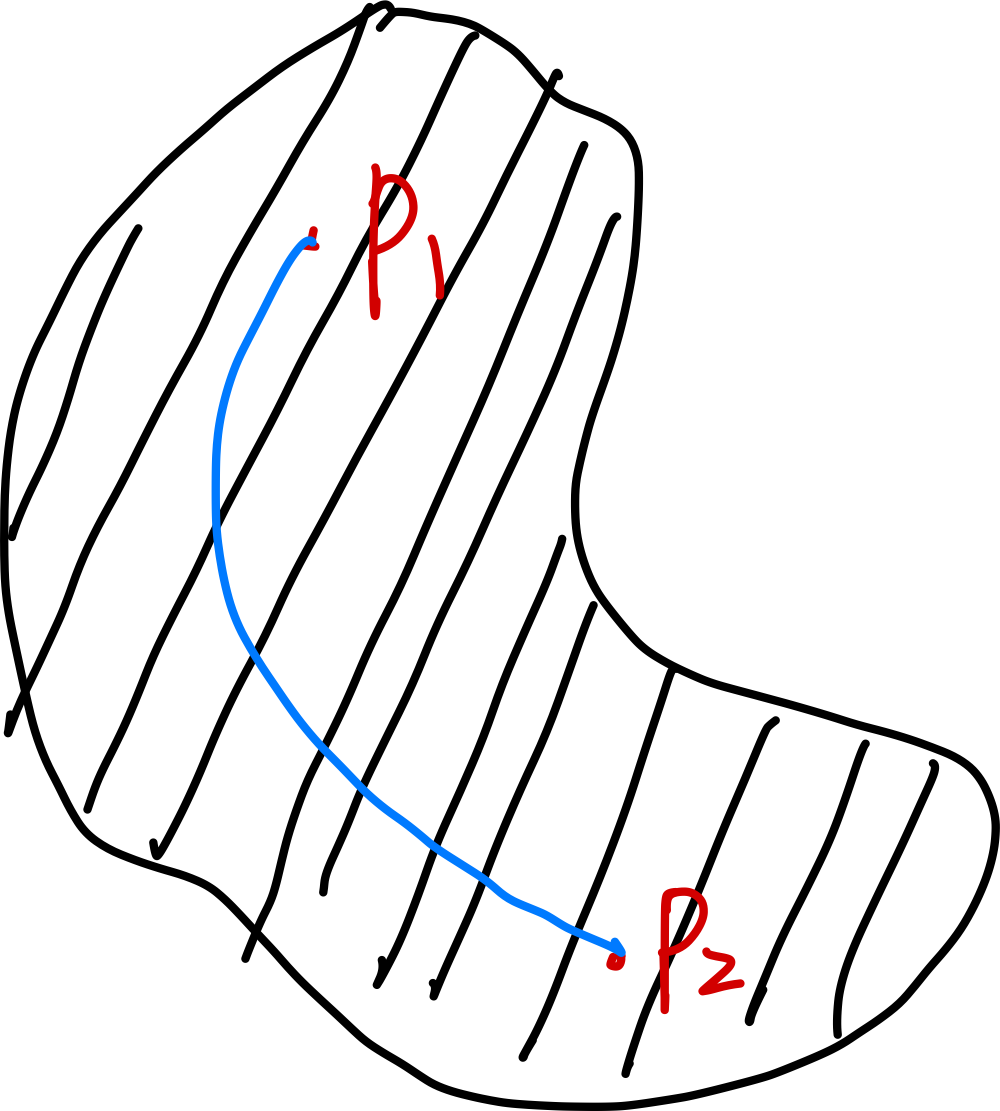
\includegraphics[scale=0.2]{"Chapter 03 images/pic1.png"}
        % \caption{}
        \label{pic1}
    \end{wrapfigure}

    元位移\(\rmd \overrightarrow{r}\)、元路程\(\rmd s\)

    则元功\(\rmd W = \overrightarrow{F} \cdot \rmd \overrightarrow{r} =
    F \cos \alpha \rmd s\)

    积分:

    \begin{align}
        W=\int_A^B \overrightarrow{F} \cdot \rmd \overrightarrow{r}=\int_A^B F \cos \alpha \mathrm{~d} s
    \end{align}

    \begin{enumerate}
        \item 功的正负
            $$
                \begin{cases}0^{\circ}<\alpha<90^{\circ}, & \mathrm{d} W>0 \\
                90^{\circ}<\alpha<180^{\circ}, & \mathrm{d} W<0 \\
                \alpha=90^{\circ}, \text{即} \overrightarrow{F} \perp \rmd \overrightarrow{r}, & \rmd W=0\end{cases}
            $$
        \item 做功的图示\\
            {
            \centering
            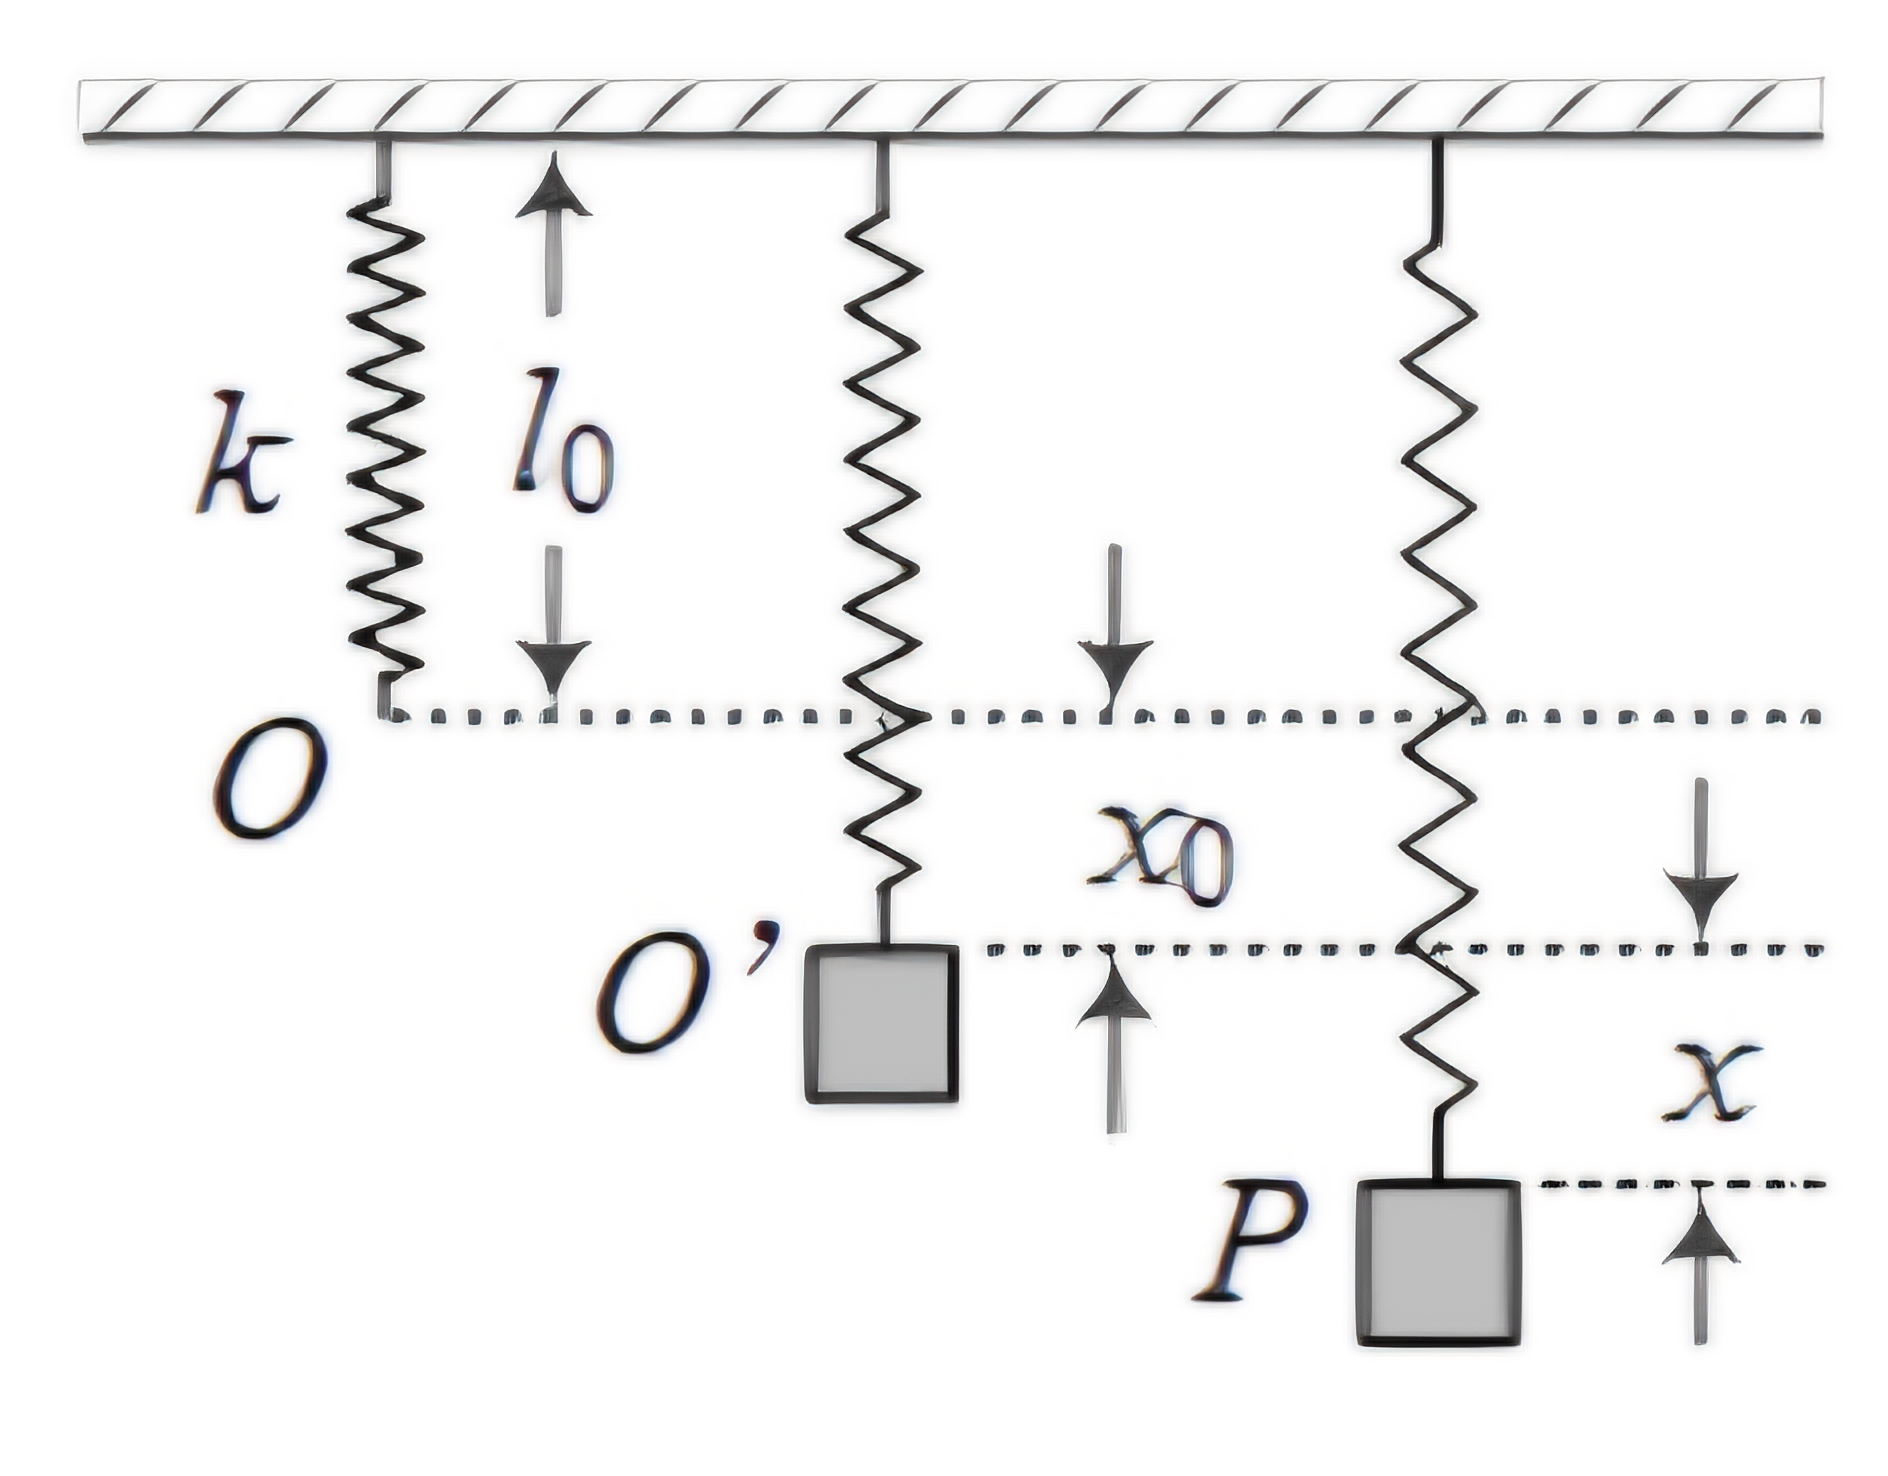
\includegraphics[scale=0.2]{"Chapter 03 images/pic2.png"}
            }
        \item 功是一个过程量,与路径有关。
        \item 合力的功,等于各分力的功的\textbf{代数和}
            \begin{align*}
                \overrightarrow{F}=F_x \overrightarrow{i}+F_y \overrightarrow{j}+F_z \overrightarrow{k} \\
                \mathrm{~d} \overrightarrow{r}=\mathrm{d} x \overrightarrow{i}+\mathrm{d} y \overrightarrow{j}+\mathrm{d} z \overrightarrow{k}
            \end{align*}
            则
            \begin{align*}
                W=\int_A^B \overrightarrow{F} \cdot \mathrm{~d} \overrightarrow{r}=
                \int_A^B\left(F_x \mathrm{~d} x+F_y \mathrm{~d} y+F_z \mathrm{~d} z\right)
            \end{align*}
            又有$W_x=\int_{x_1}^{x_B} F_x \mathrm{~d} x$、$W_y=\int_{y_1}^{y_B} F_y \mathrm{~d} y$、
            $W_z=\int_{z_1}^{z_B} F_z\mathrm{~d} z$。\\
            于是
            \[
                W = W_x + W_y + W_z
            \]

    \end{enumerate}
    
\subsection{功率}

    \textbf{平均功率}$\overline{P}=\frac{\Delta W}{\Delta t}$

    \textbf{瞬时功率}
    
    \begin{align}
        P=\lim _{\Delta t \rightarrow 0} \frac{\Delta W}{\Delta t}=\frac{\mathrm{d} W}{\mathrm{~d} t}=\overrightarrow{F} \cdot \overrightarrow{v}
    \end{align}

    即

    \begin{align}
        P = Fv\cos\alpha
    \end{align}
    
\subsection{动能定理}

\subsubsection{质点的动能定理}

    \begin{wrapfigure}{r}{4cm}
        \centering
        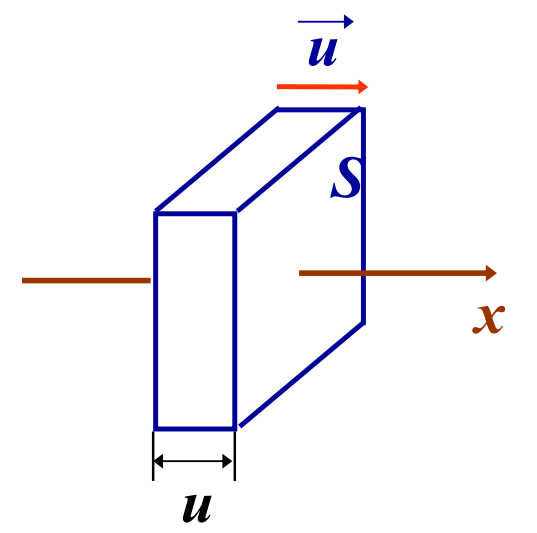
\includegraphics[scale=0.2]{"Chapter 03 images/pic3.png"}
        % \caption{}
        \label{pic1}
    \end{wrapfigure}

    $$
    \begin{aligned}
        W & =\int \stackrel{\rightharpoonup}{F} \cdot \mathrm{~d} \stackrel{\rightharpoonup}{r} \\
        & =\int F_{\mathrm{t}}|\mathrm{~d} \vec{r}|=\int F_{\mathrm{t}} \mathrm{~d} s
    \end{aligned}
    $$

    而

    $$
        F_{\mathrm{t}}=m \frac{\mathrm{~d} v}{\mathrm{~d} t}
    $$

    于是

    $$
        \begin{aligned}
        W & =\int_{v_1}^{v_2} m v \mathrm{~d} v \\
        & =\frac{1}{2} m v_2^2-\frac{1}{2} m v_1^2
        \end{aligned}
    $$

    即

    \begin{equation}
        W=\frac{1}{2} m v_2^2-\frac{1}{2} m v_1^2=E_{\mathrm{k} 2}-E_{\mathrm{k} 1}
    \end{equation}

    合外力对质点所作的功,等于质点动能的增量。——质点的动能定理

    \begin{enumerate}
        \item 功是\textbf{过程量},动能是\textbf{状态量};
        \item 功和动能依赖于惯性系的选取,但对不同惯性系动能定理形式相同。
    \end{enumerate}

\subsubsection{质点系的动能定理}

    \textbf{质点系}:由有限个或无限个质点组成的系统。(可以是固体也可以是液体,它概括了力学中最普遍的研究对象)

    \textbf{内力和外力}:质点系以外的物体作用于质点系内各质点的力称为外力,
    质点系内各质点之问的相互作用力称为内力,外力和内力的区分完全洪定于质点系(研究对象)的选取。

    \textbf{质点系内力的功}:一切内力矢量和恒等于零。但一般情烷下,所有内力作功的总和并不为零。
    例如,两个彼此相互吸引的物体,移动一段位移,都作正功。

    \textbf{质点系的动能定理}

    由质点动能定理$W=E_{k 2}-E_{k 1}=\Delta E_k$

    得

    \begin{equation}
        W_e+W_i=\sum_i\left(\frac{1}{2} m_i v_{i 2}^2-\frac{1}{2} m_i v_{i 1}^2\right)=E_{k 2}-E_{k 1}=\Delta E_k
    \end{equation}

    意义:合外力所做的功等于系统动能的增量。

\end{document}
